\documentclass[12pt]{article}

% Graphics packages
\usepackage{graphicx}
\usepackage{xcolor}
\usepackage{tikz}
\usepackage{wrapfig}
\usepackage{geometry}
\usepackage{caption}
\usepackage{subcaption}

% Environment packages


% Referencing packages
\usepackage{hyperref}
\hypersetup{colorlinks,citecolor=black,filecolor=black,linkcolor=black,urlcolor=black}

\usepackage{minted}
\usepackage[T1]{fontenc}


% Shortcuts
\newcommand{\orto}[0]{\textbf{\textcolor{red}{Orthology}}}

\setcounter{tocdepth}{4}

\begin{document}

\begin{titlepage}
    \centering
    \vfill
    {\bfseries\Large
	    \begin{flushleft}
	        \Huge TriFusion manual\\
	        \textcolor{gray}{\textbf{\normalsize Streamlining phylogenomic data gathering, processing and visualization}}
	    \end{flushleft}
    }    
    \vfill
    
    \begin{flushright}
	    by\\
		Diogo N. Silva\\
		CoBiG$^{2}$ /  cE3c\\
		University of Lisbon\\
		o.diogosilva@gmail.com
    \end{flushright}

	\begin{figure}[h]
	\centering
	\begin{subfigure}{.5\textwidth}
	  \centering
	  
\includegraphics[width=.9\linewidth]{figures/logo_ce3c.jpg}
	\end{subfigure}%
	\begin{subfigure}{.5\textwidth}
	  \centering
	  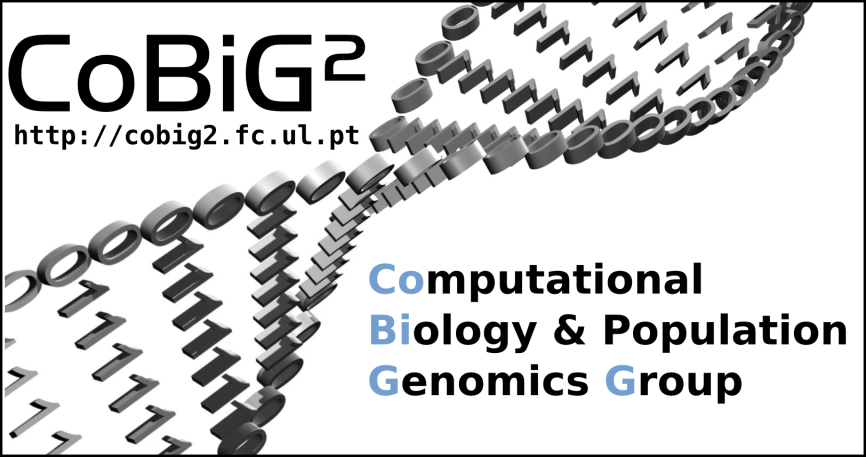
\includegraphics[width=.9\linewidth]{figures/logocobig.png}
	\end{subfigure}
	\end{figure}

\end{titlepage}

\tableofcontents

\linespread{1.5}

\pagebreak


\section{About TriFusion}

TriFusion is a GUI and command line application designed to streamline the workflow of phylogenomic projects. With the dramatic increase in size of data sets for phylogenetics and population genetics, programming has become a crucial tool to gather, process and analyze the data. However, this may still represent a hurdle that precludes the execution of such projects by a broader range of researchers. TriFusion aims to mitigate this issue by providing a user-friendly visual interface that empowers users without any programming knowledge with a set of tools and operations that can handle large sets of data.

TriFusion is an open source, cross-platform application written in Python 2.7 and using the Kivy framework.

\section{Downloading and Installing TriFusion}

Executables as available for Linux and Windows operating systems:


- Linux executable

- Windows executable

\subsection{Installation from source}

TriFusion is regularly updated with new features and bug fixes. These will eventually be bundled into the executable versions but if you wish to stay on the bleeding edge of the application's development (at the cost of potential creeping bugs), use the git version. Dependencies required to run TriFusion follow below.

Python 2.7 is required to run TriFusion. It should already be present in most Unix operating systems but not on Windows. For Windows users, I recommend installing a python distribution package (such as Anaconda) that already comes with several required python libraries. Alternatively, the vanilla Python installer can be downloaded here.

Assuming python is already installed, the following libraries are required:

\begin{itemize}
\item kivy
\item matplotlib (included in Anaconda)
\item numpy (included in Anaconda)
\item psutil (included in Anaconda)
\item scipy (included in Anaconda)
\item configparser (included in Anaconda)
\item seaborn (included in Anaconda)
\end{itemize}

These can be easily installer using pip:

\begin{minted}{shell}
pip install kivy matplotlib numpy psutil scipy seaborn
\end{minted}


\section{Getting help}


\section{Feature Overview}

TriFusion provides several features across its three main modules. Here is an overview of what it can do for you.

\subsection{Orthology}

The Orthology module of TriFusion deals with the gathering of ortholog data from proteome data, which marks the initial stages of many phylogneomic projects. 

\paragraph{Detection of putative orthologs}

Given a set of multiple proteome (protein sequence) files, TriFusion uses the OrthoMCL framework to identify putative ortholog groups. Multiple sequential runs can be executed using different inflation values, which is the most important parameter in the OrthoMCL workflow.

\paragraph{Application of filters to ortholog groups}

The OrthoMCL output includes ortholog groups with multiple copies and with no minimum taxa representation requirements. TriFusion offers filters on the maximum number of gene copies and minimum taxa representation required for an ortholog group to be selected. The effect that different values for these filters may have on the final number of orthologs can be later assessed through several plotting options.

\paragraph{Full graphical report of orthology search results}

TriFusion employs a number of diverse plotting options that allow users to get a feel for the results of the orthology search. These plots can be generated within the application with the option of changing the filters on the ortholog groups and visualize their impact on the number of orthologs on the fly. Alternatively, a full report can be issued and plots automatically generated and visualized in HTML format.

\paragraph{Ability to import multiple independent search runs}

TriFusion is able to import the main output of ortholog searches performed within TriFusion or using OrthoMCL directly. This means that multiple orthology searches can be performed independently and in different systems and their results imported into TriFusion for comparative and joint analyses.

\paragraph{Automatic conversion of ortholog groups into protein and nucleotide sequence files}

The ortholog groups identified in the search operation can be converted into protein and/or nucleotide sequence files in Fasta format, given protein and CDS data base files, respectively. These conversions can be performed at any time during the exploration of the search results.


\subsection{Process}

The Process module of TriFusion deals with the conversion and manipulation of large sets of alignment files. 

\paragraph{Handling of large alignment data matrices, made easy}

TriFusion's Process module was designed to handle large sets of data ($\geq$7k alignment files) that are commonplace in phylogneomics/population genomics projects. The sheer size of such data can be quite intimidating when thinking of how it can be processed and it may be difficult to get a feel for the data. This module aims to provide a diverse set of intuitive options that can be easily executed in order to modify and prepare these data matrices quickly and efficiently for downstream analyses. Even though all of its features are able to handle large data sets, most options can be equally useful for smaller data sets.

\paragraph{Performs basic conversion/concatenation operations}

The main operations of the Process module are the basic conversion and/or concatenation of alignment files. Several commonly used input formats are supported (Fasta, Nexus, Phylip, PyRAD .loci, Stockholm) as well as several output formats (Fasta, Nexus, Phylip, MCMCTree, Stockholm, GPhoCS, IMa2), including variations of these formats for specific downstream software.

\paragraph{A diverse portfolio of secondary operations}

Where TriFusion really shines is in the breadth of available secondary operations that can be performed along with the basic operations, perhaps because they are the most difficult (and necessary) to employ for larger data sets without programming assistance. These operations are optional but most can be easily combined in a single execution. For example, it is possible to execute the concatenation of 100 files and at the same time filter the resulting alignment so that columns with more than 75\% of missing data are excluded and code gaps in binary format at the end of the sequence matrix. Alternatively, all secondary operations have the option to save their output in a separate file instead of modifying the main output file. It's up to you. 

%If the main operation if a conversion, the secondary operations are applied independently on each input alignment. On the other hand, if the main operation is a concatenation, these operations are applied on the resulting concatenated alignment.

\paragraph{Collapsing alignments}

For downstream analyses where only unique sequences are required, TriFusion is able to collapse an alignment as a secondary operation. Here, taxa with identical sequences are effectively collapsed and represented in the output alignment as a single sequence. An auxiliary file is also created mapping the new haplotype names to the original taxa names.

\paragraph{Creating consensus alignments}

For downstream analyses that require only a single representative sequence per alignment, the consensus secondary operation is available. In this case, all sequences in an alignment will be merged into a single sequence and variation within the alignment can be handled in one of several ways available. If multiple input alignments are provided for the creation of the consensus, there is also the option to save all consensus sequences into a single file, instead of in separate files. 

\paragraph{Filters, Filters and more Filters}

Alignment filtering is one of the most important steps when processing phylogenomics data sets and this module provides several filtering options for taxa, codon positions, missing data and sequence variation:

\begin{itemize}
\item Taxa filter: Input alignments can be filtered depending on whether they contain or exclude a user-provided taxa group
\item Codon filter: For protein-coding nucleotide sequences, alignments can be filtered in order to exclude certain codon positions
\item Missing data filter: This filter can be applied both within alignments or among a set of alignments. Within an alignment, it is possible to remove columns that contain a proportion of gaps (usually "-") and/or missing data (usually "N") above user-defined thresholds. Among alignments, it is possible to remove ones that contain less taxa than minimum number allowed by the user.
\item Variation filter: Input alignments can be filtered when they contain a number of variable and/or informative sites outside the range specified by the user.
\end{itemize}

\paragraph{Gap coding}

When the information contained in the indel pattern of an alignment may be of use for downstream analyses, the Gcoder secondary operation can be used. Here, the method described in Simmons and Ochoterena (2000) is employed to transform indel patterns into a binary matrix that is appended to the end of the sequence data. This operation can only be performed when the output format is Nexus.

\paragraph{Creation of data subsets}

The operations of the Process module need not be only applied to the complete data set that is currently loaded into the application. With a single click, individual alignment files or taxa can be toggled out of the active data set and ignored from subsequent operations. This can be very useful when, for example, a complete data set includes mitochondrial and nuclear genes and the user wishes to concatenate all genes, then only the mitochondrial genes, and finally only the nuclear genes. Likewise, it is possible to exclude certain groups of taxa from some operations. For larger or more complex scenarios, TriFusion provides creation dialogs that allows the definition of subsets of alignments and/or taxa, which can be easily switched.

\paragraph{Set gene partitions, codon partitions and substitution models}

Gene partitions are fully customizable within the application or by importing partition schemes. For nucleotide sequences, all possible combinations of codon partitions can be specified along with the substitution model for each partition. This information is then saved on the output formats that support this information (Nexus and Phylip partition file).

\paragraph{Revert a concatenated alignmnet}

A previously concatenated alignment can be reverted to its individual and separate files using the revert concatenation option, by providing information on its partitions. These partitions may be already defined in the alignment file (Nexus format), imported from a separate file with partitions definitions, or defined within the application.


\paragraph{Concatenation of alignment weight files}

Many modern phylogenetic software support the attribution of weights to each alignment column as a measure of uncertainty from the alignment procedure. This alignment column weights can be obtained using software such as Zorro. However, there is usually lack of support when concatenating multiple alignment files with their corresponding weight files. TriFusion offers the option to joint concatenate alignment files and their corresponding weight files in an easy way. 

\subsection{Statistics}

Because figures may be worth a thousand words, the Statistics module offers a diverse set of plotting and statistical options that allows users to quickly and easily visualize many aspects of their data set. In other words, it lets you get a feel for the data, painlessly. These plotting options are sorted into four main categories: General information; Polymorphism and variation; Missing data; Outlier detection.

\paragraph{Visualize your data set focusing on single genes, taxa or genes}

For the majority of the plotting options, there are more than one way to look at the data. For example, when you wish to investigate the sequence similarity of your data set, this information can be displayed focusing on: (i) a single gene, using a sliding window approach; (ii) taxa, using a triangular heat matrix; (iii) gene average, using a distribution of sequence similarity values across all genes. Moreover, the active data sets can also be modified, as in the Process module, and all plots will be updated according to the new active data sets.

\paragraph{Get summary statistics and general alignment information instantly}

After loading an alignment data set into TriFusion, the first operation performed by the Statistics module is to compute several summary statistics and general gene information unobtrusively in the background. When the calculations are done, they are revealed in the main Statistics screen. 

\paragraph{General information plots}

The general information category offers plotting options with information on the distribution of sequence size, proportion of nucleotides/residues, and distribution of taxa frequency.

\paragraph{Polymorphism and variation plots}

The polymorphism and variation category focus on plotting options that investigate the amount and distribution of sequence variation found in the alignment data set. The user may investigate the pairwise sequence similarity, number and distribution of segregating sites and compute the allele frequency spectrum (only for nucleotide alignments). An additional operations calculates the correlation coefficient between the length and sequence variation of the alignments.

\paragraph{Missing data plots}

Missing data plots allows the user to investigate the amount and distribution of missing data in the data set. The plotting options include a gene occupancy plot, which allows a quick visualization of the amount of missing genes/taxa in the data set, distributions of missing taxa and data, and the cumulative distribution of missing genes to assist the user on the best minimum taxa representation threshold that maximizes the amount of data and minimizes the missing data.

\paragraph{Outlier detection plots}

Outlier detection plots will assist the user in the identification of taxa or genes with outlier characteristics, which may be indicatives of problems during the creation of the alignment data set. Outlier taxa or genes can be identified based on the sequence length, number of segregating sites and amount of missing data.

\paragraph{Publication ready figures and tables}

For nearly all options it will be possible to export the current plot as a figure, in a number of output formats, as well as in table format (in .csv). These plots have been extensively customized in order to be of high quality and publication ready and include the option to convert into black and white versions.

\paragraph{Plot fast switching}

Some plotting options may take a while to complete, depending on the size of the active data set. To reduce waiting times, a number of techniques were employed to allow fast switching between plots that were already generated. In addition, costly computations are usually stored in SQLite data bases to reduce computing times when changing the active data set.


\section{TriFusion Interface}

\subsection{Import data}

\subsection{Creating data sets}

\subsection{Project management}


\section{Orthology module - GUI}

The Orthology module is able to perform two distinct operations: \textbf{\textit{Search}} and \textbf{\textit{Explore}}. 

Using the \textbf{\textit{Search}} operation it is possible to search for potential ortholog groups from a set of multiple proteome files in Fasta format using the framework of OrthoMCL. Several parameters can be changed by the user, such as filters for the maximum number of genes copies allowed or the minimum number of taxa represented in an ortholog group, and the inflation values for the MCL analysis. The main output of this operation will be the creation of a directory containing the unaligned sequence files for each ortholog group, and a file containing information on the sequences of all ortholog clusters. This file is the main output of OrthoMCL and is called a groups file. Multiple groups files can be created in a single Search run by specifying a range of inflation values. These can be later provided as input to the \textit{\textbf{Explore}} operation for comparison and investigation of the results.

The \textbf{\textit{Explore}} operation allows users to compare different runs of the \textbf{\textit{Search operation}}, modify filters and visualize different aspects of the obtained ortholog groups. During this investigation, it is possible to evaluate the effect of the cluster filters on several parameters (missing data, gene copies, etc) and at any point the users will have the option to export the orthologs with the current filters as protein or nucleotide sequences.

\subsection{Search operation}

\subsubsection{Import data}

The required input for the Search operation are proteome files in Fasta format, one for
each taxon. Data files can be loaded into the application as described in [XXXX]. 
TriFusion will interpret the name of the proteome file (minus extension) as
the taxon name, so it is recommended that these files are named accordingly. Within each
Fasta proteome file, there is only one requirement. Assuming that the headers for each
sequence have one or more fields separated by a ``|'' symbol, at least one of these fields
must be unique and different among all sequences.  TriFusion will automatically detect
that field for you and show a warning if there are no unique fields. Consider the example:

\begin{minted}{shell}
>Homo_sapiens|predicted protein|231
AGT(...)
>Homo_sapiens|predicted protein|232
ATG(...)
>Homo_sapiens|apolipoprotein E|233
ATG(...)
\end{minted}

This is a well formatted Fasta file with headers containing three fields, the third
one being the unique ID field.

\subsubsection{Search operation main options}

\paragraph{Threads}

Set the maximum number of CPU's that will be used during the All-vs-All search. TriFusion
was designed to use USEARCH to perform this step instead of NCBI's BLASTp, since it
provides almost identical results in a fraction of time [See section on USEARCH vs.
BLASTp]. To avoid specifying more CPU's than those available, TriFusion automatically
detects the number of CPU's in the current system and sets them as the maximum value.

\paragraph{Ortholog filters}

Set the filters on the maximum number of gene copies and minimum number of taxa
represented per ortholog group, to be applied at the end of the Search operation.


\subsubsection{Search operation additional options}



\section{Orthology module - Command line}

\section{Process module - GUI}

\section{Process module - Command line}

\section{Statistics module - GUI}

\section{Statistics module - Command line}



\bibliography{}
\bibliographystyle{plain}

\end{document}
